\chapter{Zaimplementowany system wspomagający autonomiczne lądowanie drona}
\label{cha:opis_implementacji}
%TODO Tu będzie początek tego nowego rozdziału. Przed modelem programowy proszę kilka zdań wstępu (co bedzie w treści)
W~rozdziale omówiono zagadnienia związane ze~szczegółami implementacji systemu. Ważną rolę w~tworzeniu kolejnych modułów odegrał model programowy, czyli program napisany w~dowolnym języku programowania i~wykonywany na~komputerze~PC, którego działanie oddaje funkcje modułu tworzonego w~sprzęcie. Porównanie wyników działania modelu programowego i~symulacji modułu daje informację o~poprawności implementacji. Model programowy wraz z~uzasadnieniem użycia poszczególnych modułów przedstawiono na~początku rozdziału.\\
Następnie opisano wszystkie części przetwarzania sygnału, od~przesłania obrazu przez kamerę, do~wysyłania komend do~autopilota.
\section{Implementacja i ewaluacja modelu programowego}
\label{sec:implementacja_modelu_programowego}
Model programowy został napisany w pakiecie Matlab przy wykorzystaniu funkcji dostępnych w~bibliotece \textit{Image Processing Toolbox}. 
Pozwoliło to~na~szybkie prototypownie systemu wizyjnego, składającego się~z:
%TODO Przedstawić ogólny schemat algorytmu oraz go skórtowo omówić.
\begin{itemize}
	\item konwersji z~przestrzeni RGB do YCbCr,
	\item binaryzacji ze~stałymi progami,
	\item mediany,
	\item otwarcia,
	\item indeksacji jednoprzebiegowej wyznaczającej pole powierzchni i~prostokąt otaczający obiektów.
\end{itemize}
Piksel w~przestrzeni barw YCbCr opisują trzy składowe: Y (luminancja), Cb (chrominancja, która wyraża różnicę między luminancją, a~kolorem niebieskim) oraz Cr (chrominancja, która wyraża różnicę między luminancją,~a~kolorem czerwonym). \\
Zaletą stosowania tej przestrzeni barw jest oddzielenie sygnału luminancji od~sygnałów chrominancji, pozwalające na~dokonywanie przetwarzania sygnału przy mniejszej zależności od~oświetlenia.\\
Zastosowanie binaryzacji pozwala na~oddzielenie znacznika od~tła. Na~wyjściu modułu znajdują się tylko dwa rodzaje pikseli: należące i~nienależące do~obiektu (Rys. \ref{fig:bin_1}).
Na~obrazie często znajdują się jednak inne niewielkie obszary (zakłócenia), które zostały wykryte. Pozostawienie ich na~wejściu modułu indeksacji zwiększyłoby niepotrzebnie liczbę nadawanych etykiet, która jest ograniczona (sekcja \ref{subsec:indeksacja}).\\
Częściowym rozwiązaniem problemu jest zastosowanie mediany. Jest to~operacja kontekstowa, w~której pikselowi wyjściowemu przypisuje się wartość środkową uporządkowanego zbioru wartości pikseli z~otoczenia piksela wejściowego. \\
Wykorzystanie mediany powoduje znaczne zmniejszenie błędnych obszarów, jednakże niekiedy na~obrazie obecne są~nadal małe grupy białych pikseli nienależących do~obiektu (Rys. \ref{fig:median_1}).\\
Z~tego powodu zdecydowano się na~wykorzystanie erozji. Erozja i~dylatacja to~operacje morfologiczne, w~których pikselowi wyjściowemu przypisuje się wartość odpowiednio najmniejszego i~największego piksela w~sąsiedztwie piksela wejściowego. Sąsiedztwo piksela określa kształt i~rozmiar elementu strukturalnego.  
Zastosowanie morfologicznego otwarcia, składającego się z~erozji i~dylatacji, pozwala niekiedy na~całkowite wyeliminowanie błędnych białych pikseli (Rys. \ref{fig:opened_1}).
Indeksacja jednoprzebiegowa to~operacja pozwalająca na wyodrębnienie z~obrazu cech poszczególnych obiektów. Obiekty rozumiane są~jako grupy połączonych ze~sobą pikseli. Ze~względu na~wykorzystywany współczynnik kształtu obliczano prostokąt otaczający i~pole obiektów. 
\begin{figure}
	\centering
	\begin{subfigure}{0.7\textwidth}
		\centering
		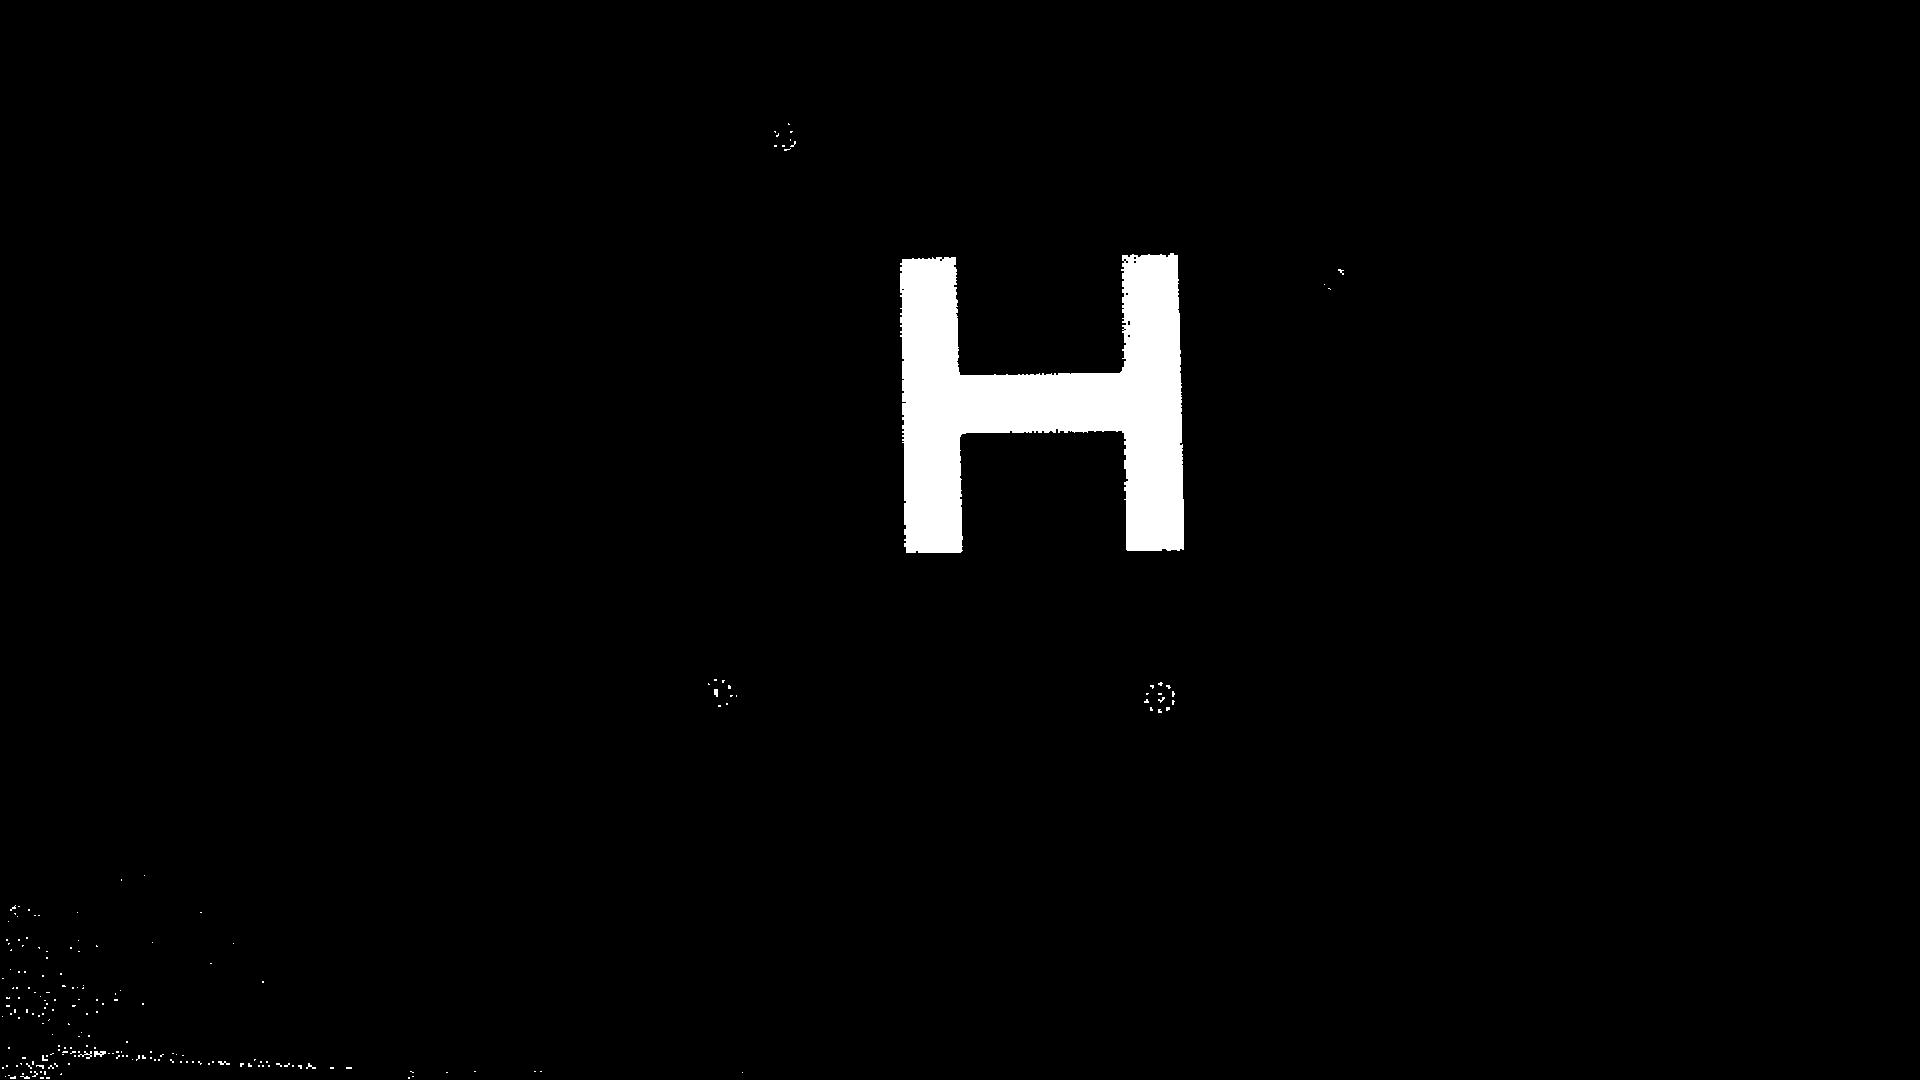
\includegraphics[width=\textwidth]{bin.jpg}
		\caption{Rezultat binaryzacji.}
		\label{fig:bin_1}
	\end{subfigure}
	\begin{subfigure}{0.7\textwidth}
		\centering
		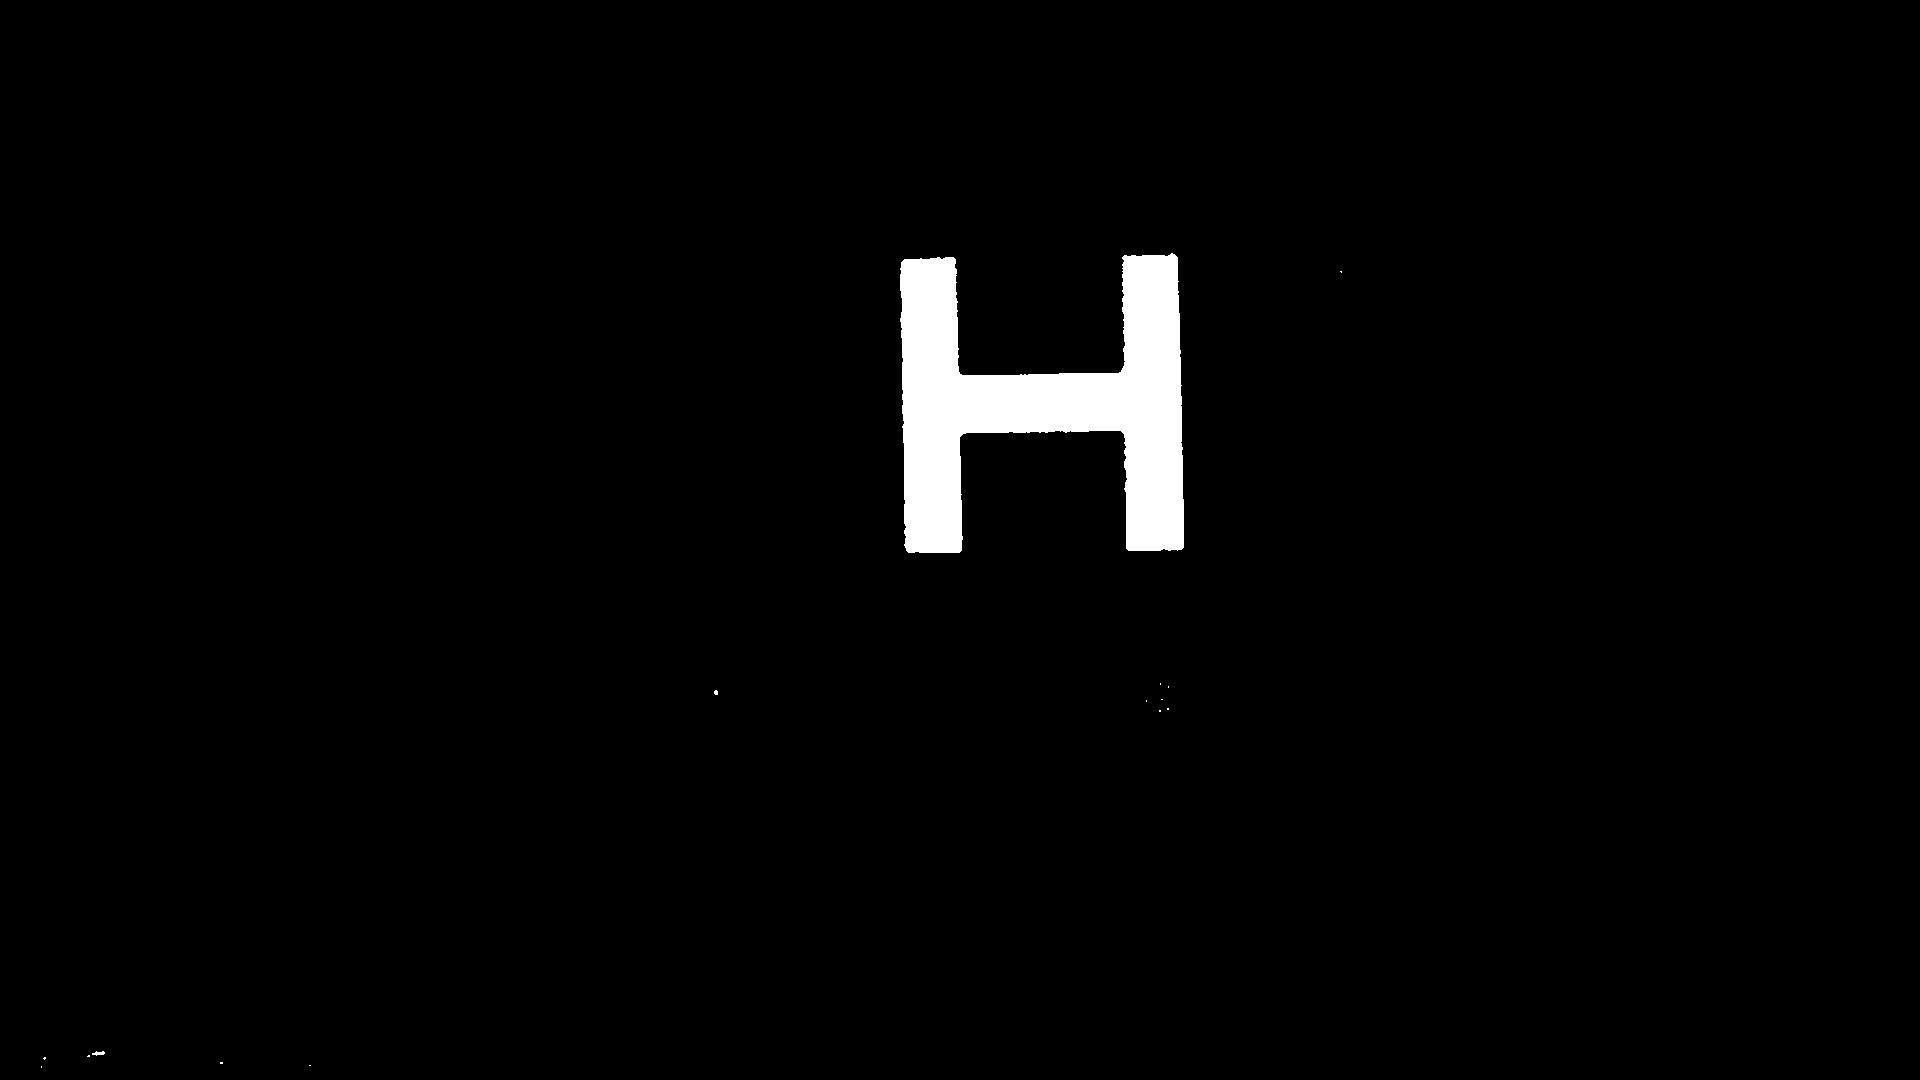
\includegraphics[width=\textwidth]{median.jpg}
		\caption{Obraz po medianie}
		\label{fig:median_1}
	\end{subfigure}\\
	\begin{subfigure}{0.7\textwidth}
		\centering
		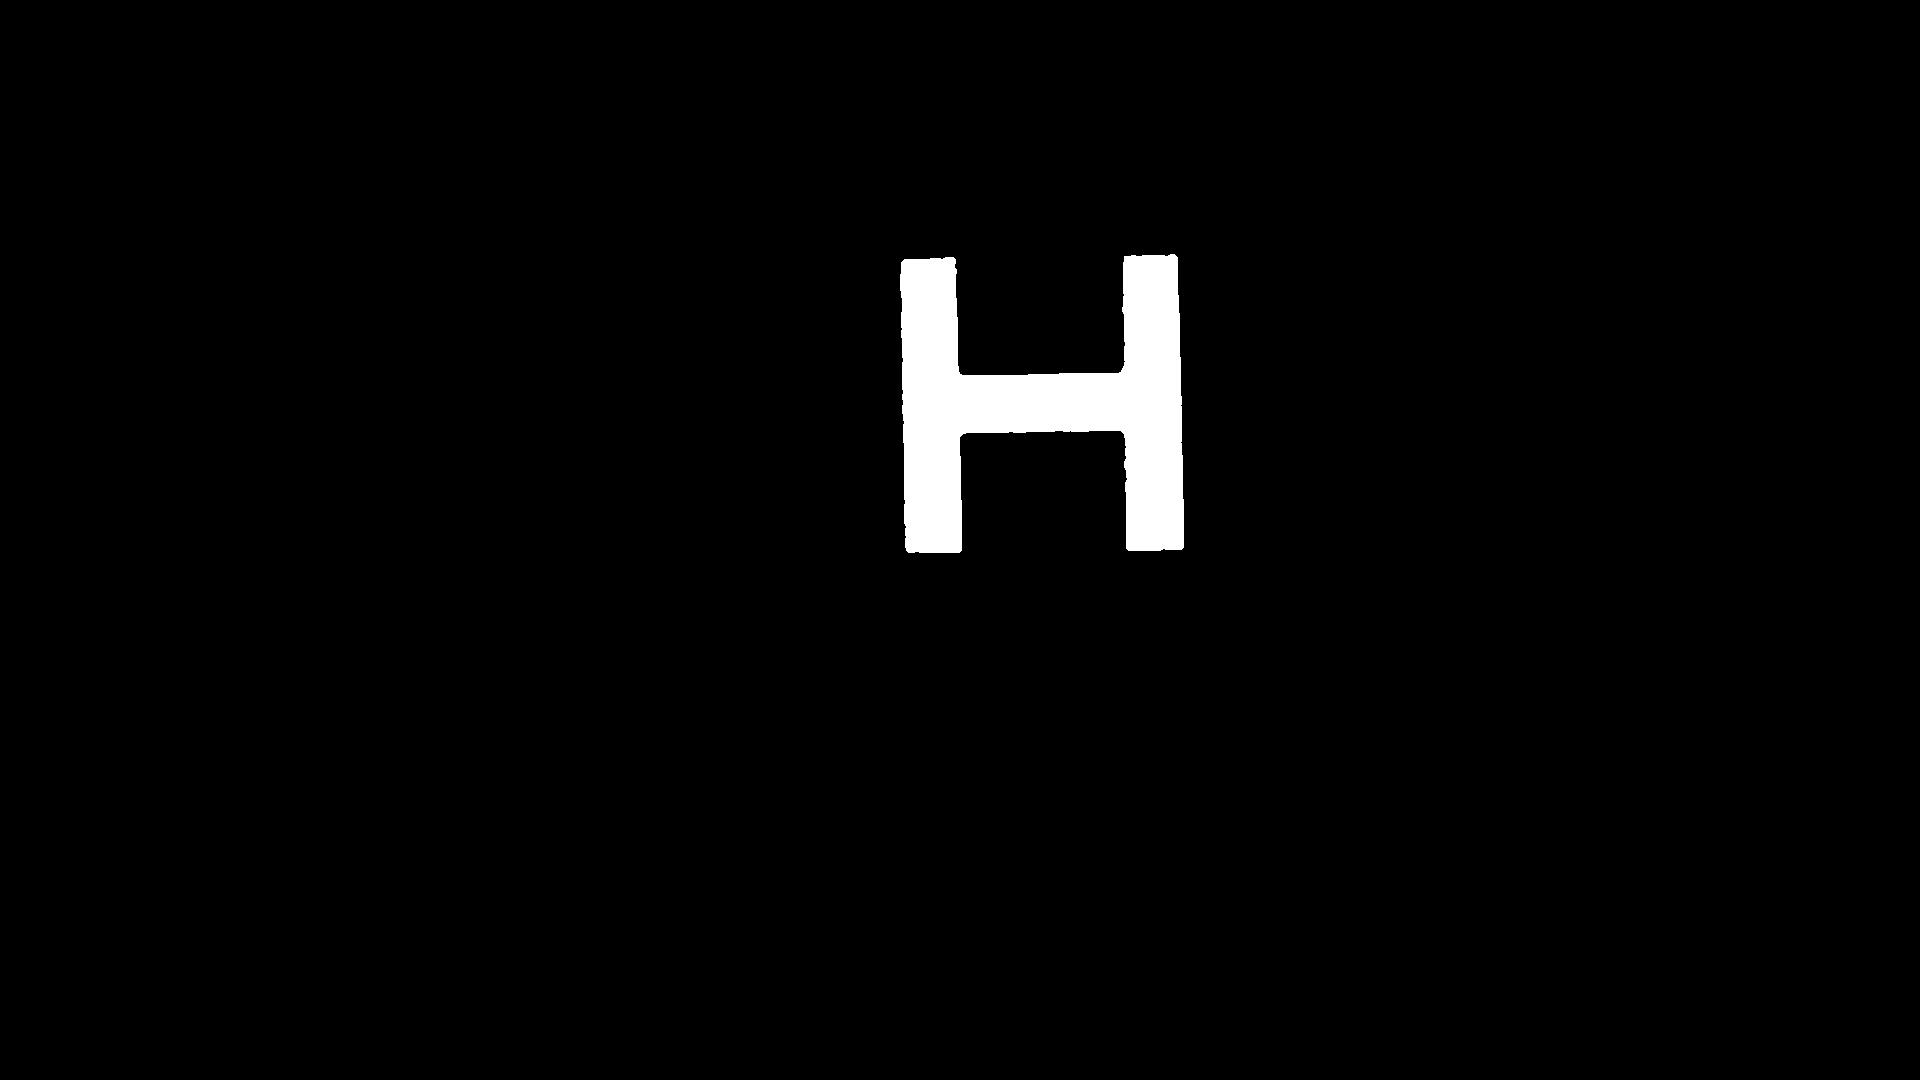
\includegraphics[width=\textwidth]{opened.jpg}
		\caption{Wynik otwarcia}
		\label{fig:opened_1}
	\end{subfigure}
	\caption{Przykładowe rezultaty binaryzacji, mediany i~otwarcia}
	\label{fig:operacje}
\end{figure}
%TODO jest niejasne...bo jest mieszanie HW i modelu. Może proszę napisać dwa zdania o sekwencjach, bo chyba Pan zaczął od zwykłych, a potem z PCAM. Natomiast sprawę PCAM proszę "załatwić" w ten sposób, że ten opis ponież w części SW (jakiś subsectio), a tu się powołać

%TODO W kolejnych podrozdziałch uzasadnienie wyboru poszczególnych komponentów. Treść z "testy".(uzasadnienie dałem w części o modelu)

\subsection{Akwizycja ramek na kartę SD}
Aby możliwe było wprowadzanie ramek obrazu do modelu, należało umożliwić akwizycję obrazów na~kartę~SD. W~pobranym projekcie zastosowano połączenie toru wizyjnego AXI z~pamięcią procesora. Połączenie realizuje moduł AXI Video Direct Memory Access. Informacja o~miejscu w~pamięci, gdzie zapisywane są~ramki podawana jest przy inicjalizacji połączenia na~terminal. \\
W~celu umożliwienia komunikacji z~kartą uaktywniono interfejs procesora SD0. Następnie do~projektu w~SDK dodano bibliotekę ,,xilffs'' i,~korzystając z~funkcji systemu plików opisanych w~\cite{xilffs}, napisano zapis ramek do~pliku. 
Ze~względu na~prostotę pliku zdecydowano~się na~format ppm. W~formacie nie występuje żadna kompresja i~jest on~nieefektywny pod~względem zapotrzebowania na pamięć. Niemniej jednak, dysponując odpowiednio dużą ilością miejsca na~karcie i~chcąc w~łatwy sposób zapisać dane, wybrano właśnie ten format. Zapis danych w~formacie ppm jest prosty, gdyż plik składa się jedynie z~nagłówka (typ pliku, rozmiary obrazka, maksymalna wartość składowych) oraz kolejnych wartości w~formie pojedynczych bajtów (jeśli maksymalna wartość jest mniejsza niż 256).  \\
%TODO Ten opis powyżej trzeba nieco rozwinąć.(wykonane)

%W~późniejszym stadium projektu, z~powodu różnic na obrazie zapisywanym na kartę i~wyświetlanym na ekranie, zdecydowano się na zmianę tej koncepcji.  %TODO chyba na kartę.
%TODO a co to za róznice.
%Zaimplementowano cały tor wizyjny w~części PL układu Zybo Z7-20 i~przechwytywano przetworzone obrazy wyświetlane na~monitorze. 
%Dzięki takiemu podejściu podczas testowania widziano rzeczywiste wyniki przetwarzania.

\section{Implementacja sprzętowo-programowa}
\label{sec:implementacja_sprzetowo_programowa}
Na Rys. \ref{fig:system} przedstawiono ogólny schemat implementacji systemu. Na~niebiesko zaznaczone zostały komponenety sprzętowe, na~żółto oznaczono moduły zaimplementowane w~części rekonfigurowalnej, natomiast na~zielono zaznaczono system procesorowy. Z~kamery trafia do~układu sygnał wizyjny, który następnie jest przetwarzany przez poszczególne moduły. Po~wyborze znacznika informacja o~jego pozycji i~uchybie regulacji trafia do~procesora. System procesorowy wysyła komendy sterujące do~autopilota. Zadaniem układu regulacji jest przesunięcie drona nad~lądowisko, umożliwiając wykonanie lądowania.
W~dalszej części rozdziału omówiono poszczególne komponenty systemu.   
%TODO Krótki wstęp np. ogólny scheamt implementacji ze wskazaniem na podział HW/SW, taki schemat sprzętu (z peryferiami). Potem będzie Pan omawiał poszczególne komponenty. (wykonane)
\begin{figure}[h]
	\centering
	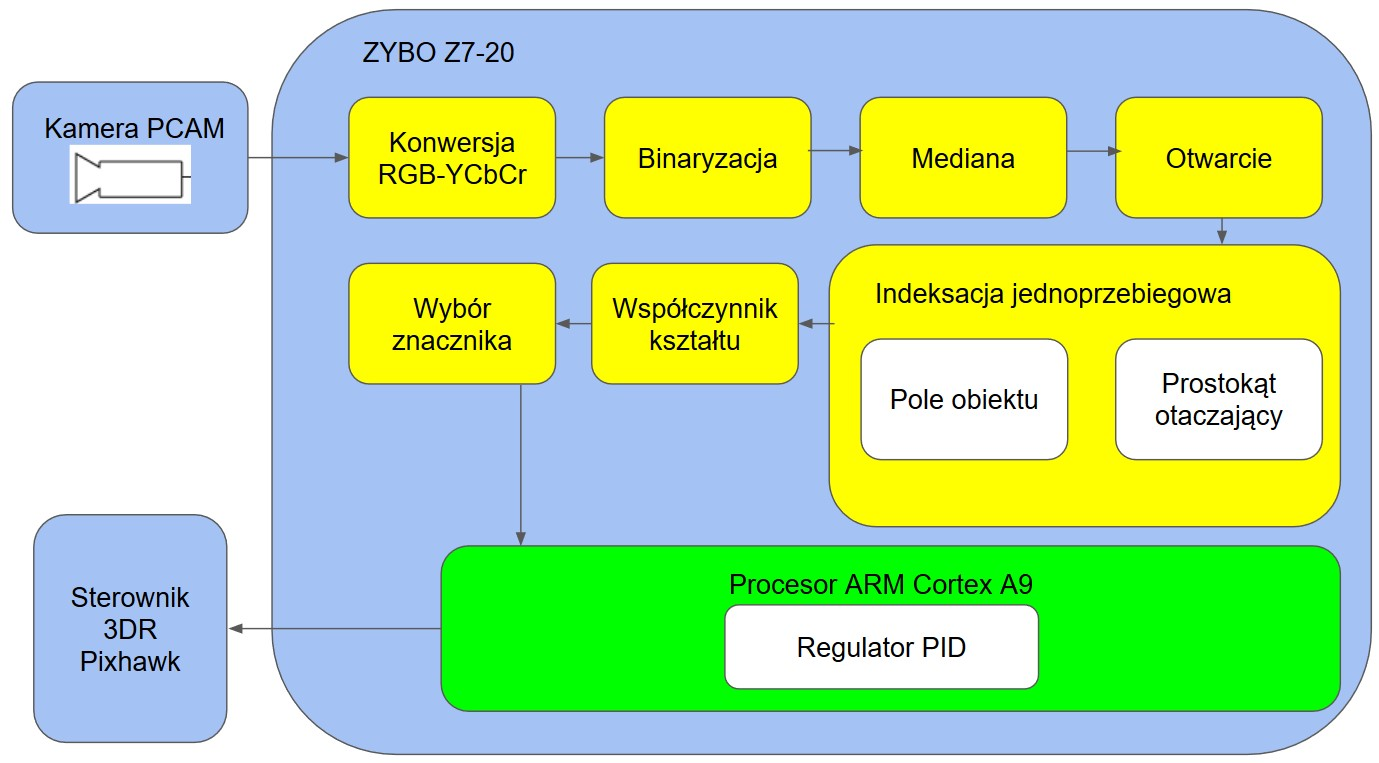
\includegraphics[width=\textwidth]{system.jpg}
	\caption{Schemat przedstawiający zaimplementowany system.}
	\label{fig:system}
\end{figure}  
\subsection{Integracja kamery i płytki}
\label{sec:integracja_uklad_kamera}
Producent na swojej stronie internetowej zapewnia projekt demonstracyjny połączenia kamery i~płytki~\cite{projektPCAM}. Przez port szeregowy możliwa jest zmiana rozdzielczości, szybkości akwizycji ramek, współczynnika korekcji gamma, ustawień balansu bieli. Możliwe są~następujące opcje dotyczące dwóch pierwszych parametrów:
\begin{itemize}
	\item 1280 x 720, 60 fps,
	\item 1920 x 1080, 15 fps,
	\item 1920 x 1080, 30 fps.
\end{itemize}
Okazało się również, że dla rozdzielczości 1280 x 720 większy jest kąt widzenia kamery. Ze~względu na~powyższy fakt oraz przyspieszenie obliczeń, zdecydowano się na~najmniejszą dostępną rozdzielczość.\\
Przeprowadzanie syntezy i~implementacji projektu możliwe było przy użyciu darmowego oprogramowania Vivado oraz SDK w wersji WebPack -- używano wersji~2018.2. \\
Pobrany projekt stanowił bazę do dalszych prac.
\subsection{Konwersja z przestrzeni barw RGB do YCbCr}
\label{subsec:konwersja}
Konwersję z przestrzeni barw RGB do YCbCr wykonano zgodnie ze wzorem \ref{eq:ycbcr}. 
Przy implementacji wykorzystano sprzętowe mnożarki oraz sumatory. Na~Rys. \ref{fig:drzewo_ycbcr} przedstawiono schemat operacji arytmetycznych dla jednej ze~składowych. Aby możliwe było prowadzenie obliczeń, wszystkie stałe należało przedstawić w~postaci liczb stałoprzecinkowych. Do~reprezentacji stałoprzecinkowej użyto rejestrów o~szerokości 18~bitów.
\begin{equation}
\label{eq:ycbcr}
\begin{bmatrix} Y \\ 
Cb\\
Cr
\end{bmatrix}=
\begin{bmatrix} 0,299 & 0,587 & 0,114\\ 
-0,168736 & -0,331264 & 0,5\\
0,5 & -0,418688 & 0,081312
\end{bmatrix}
\begin{bmatrix} R\\
G\\
B
\end{bmatrix}+
\begin{bmatrix} 0\\
128\\
128
\end{bmatrix}
\end{equation}

%TODO Może schemat ?(wykonane)
\begin{figure}[h]
	\centering
	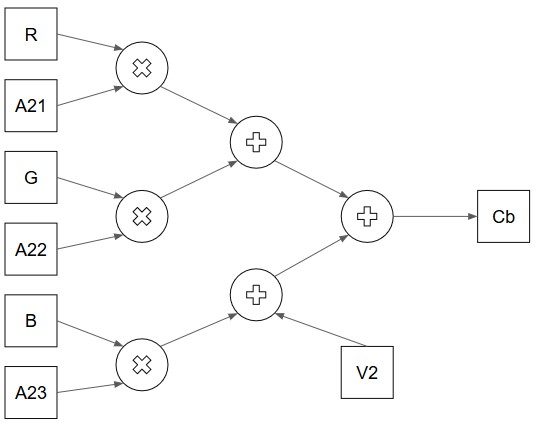
\includegraphics[width=0.7\textwidth]{drzewo_ycbcr.jpg}
	\caption{Schemat wyznaczania składowej Cb. $A21=-0,168736, A22=-0,331264, A23=0,5, V2=128$.}
	\label{fig:drzewo_ycbcr}
\end{figure} 

\subsection{Binaryzacja}
\label{subsec:Binaryzacja}
% dobieranie progu: 2 multiplekser sterowany buttonem?
Piksel wyjściowy otrzymywał wartość maksymalną (kolor biały), jeśli wartości Cb i~Cr mieściły się pomiędzy wyznaczonymi eksperymentalnie progami.  
W~innym przypadku pikselowi przypisywana była wartość 0 (kolor czarny). 
Do~szybkiej zmiany progów wykorzystano komunikację PS-PL z~wykorzystaniem rejestrów AXI - progi mogły być zmieniane z~poziomu terminala i~testy nie wymagały ponownych implementacji.  

%TODO Prawda jest taka, że to najlepiej zrobić z wykorzystaniem rejestrów AXI - to jest to przerobienia w kolejnej iteracji.(wykonane)


\subsection{Mediana}
\label{subsec:Mediana}
% obrazek wyznaczania kontekstu
% obrazek drzewa sumacyjnego

W~przypadku działania na~obrazie binarnym operacja mediany może być przeprowadzona przez obliczenie sumy wartości pikseli wewnątrz kontekstu, a~następnie porównanie jej z~połową maksymalnej wartości tej sumy. 
Ze względu na łatwość implementacji oraz zadowalające wyniki filtracji, zdecydowano się na~rozpatrywanie kontekstu w~kształcie kwadratu o~boku 5~pikseli. 
Spowodowało to~konieczność zapamiętywania kontekstu piksela w~25 rejestrach oraz 4~linii obrazu w długich liniach opóźniających zbudowanych w~oparciu o~pamięć BRAM.
Schemat wyznaczania kontekstu przedstawiono na rysunku \ref{fig:kontekst}. 
Sygnały synchronizacji zostały doklejone do wartości piksela i~w~przedstawionej strukturze przesuwają się razem z~nim. 
Sumę wyliczano w~2~etapach, dodając najpierw elementy w~wierszach, potem sumując wyniki (Rys. \ref{fig:drzewo_sumacyjne}).
%Latencja modułu wynosiła 2, należało zatem opóźnić sygnały synchronizacji o~tyle taktów zegara. 
%TODO Modułu to więcej bo 4 linie i trochę.
\begin{figure}[h]
	\centering
	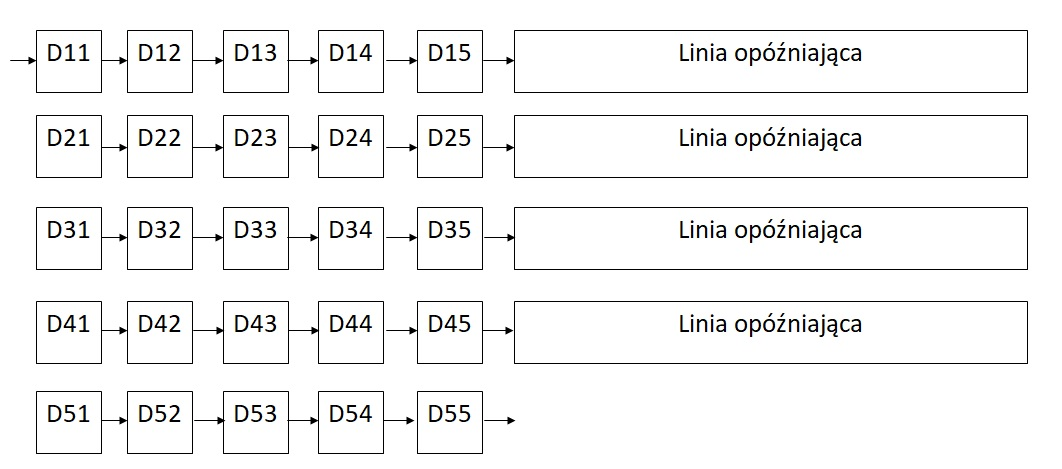
\includegraphics[width=\textwidth]{kontekst.jpg}
	\caption{Schemat wyznaczania kontekstu dla mediany, erozji i dylatacji.}
	\label{fig:kontekst}
\end{figure}  
\begin{figure}[h]
	\centering
	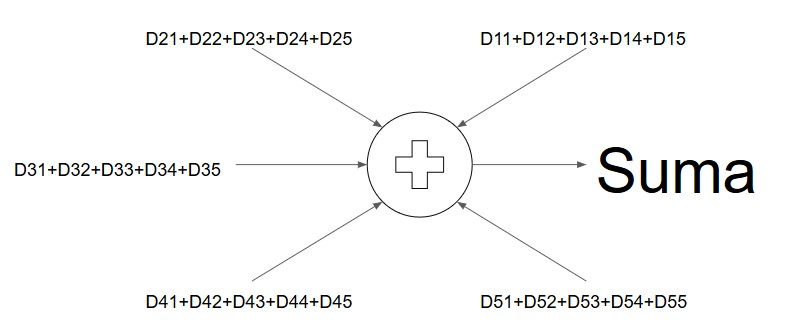
\includegraphics[width=\textwidth]{drzewo_sumacyjne.jpg}
	\caption{Schemat wyznaczania sumy otoczenia piksela.}
	\label{fig:drzewo_sumacyjne}
\end{figure}  

\subsection{Erozja i dylatacja}
\label{subsec:erozja}
Podobnie jak w~przypadku mediany, jako element strukturalny zdecydowano się na~kwadrat o~boku 5~pikseli. 
Moduł erozji ustawia wartość piksela wyjściowego na~maksymalną wartość, gdy~w~sąsiedztwie znajdują się same białe piksele. 
W~module dylatacji zwracana jest wartość maksymalna, gdy~przynajmniej jeden piksel w~sąsiedztwie ma~wartość maksymalną.
%Latencja modułów wynosi~1. 
%TODO Jw. skoro kontkst to 4 linie i trochę...

\subsection{Prostokąt otaczający i pole powierzchni}
\label{subsec:prostokat_otaczajacy}

Znalezienie prostokąta otaczającego sprowadza się do wyznaczenia skrajnych jego punktów na górze, dole, po lewej oraz prawej stronie. Na podstawie sygnałów synchronizacji oraz wymiarów obrazka wyznaczano współrzędne aktualnie przetwarzanego piksela. 
Jeśli jest to piksel należący do obiektu, następuje inkrementacja jego pola powierzchni. Do~odpowiednich rejestrów trafiają wówczas również wartości współrzędnych piksela, jeśli wykraczają poza aktualną zawartość rejestrów:
\begin{itemize}
	\item do~rejestru zawierającego górny bok prostokąta trafi współrzędna wierszowa, jeśli będzie ona mniejsza od aktualnej,
	\item do~rejestru zawierającego dolny bok prostokąta trafi współrzędna wierszowa, jeśli będzie ona większa od aktualnej,
	\item do~rejestru zawierającego lewy bok prostokąta trafi współrzędna kolumnowa, jeśli będzie ona mniejsza od aktualnej,
	\item do~rejestru zawierającego prawy bok prostokąta trafi współrzędna kolumnowa, jeśli będzie ona większa od aktualnej,
\end{itemize}  %TODO to by można opisać bardziej prezycyjnie (wykonane)
Obliczeń pola powierzchi i~współrzędnych prostokąta otaczającego nie~wykonywano w~oddzielnym module, lecz stanowiły one część modułu indeksacji.

\subsection{Indeksacja}
\label{subsec:indeksacja}

%TODO role tej indekscji trzeba opiać w częsci o modelu. Już nie wspomnę, że nie było o niej mowy... Musi Pan napisać po co to Pan robił.

Zazwyczaj na wejście modułu indeksacji podawany jest obraz zbinaryzowany, natomiast na~wyjściu pojawia się obraz, na którym  wartość  pikseli odpowiada przypisanej do~danego obiektu etykiecie. 
Rozważane jest otoczenie każdego piksela, składające się z trzech pikseli nad nim oraz jednego po~lewej stronie, tak jak zostało to przedstawione na rysunku \ref{fig:ind_sasiedztwo}. 
Indeksacji dokonuje się bezpośrednio na~obrazie wejściowym. 
Podczas iteracji po wszystkich pikselach, w~przypadku znalezienia piksela należącego do któregoś z~obiektów, może zajść jeden z~trzech przypadków:
\begin{enumerate}[label=(\alph*)]
	\item w otoczeniu piksela znajdują się tylko piksele należące do tła,
	\item otoczenie zawiera jeden lub więcej pikseli, którym została wcześniej przypisana taka sama etykieta~$L$,
	\item w otoczeniu znajdują się piksele posiadające różne etykiety.
\end{enumerate} 
\begin{figure}[h]
	\centering
	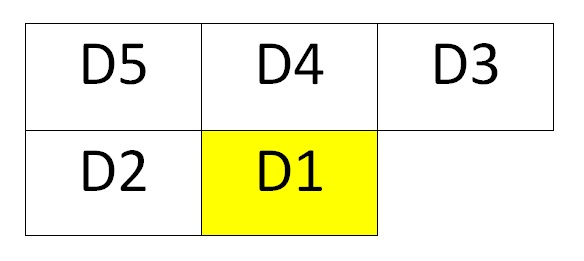
\includegraphics[width=0.5\textwidth]{ind_sasiedztwo.jpg}
	\caption{Sąsiedztwo piksela brane pod uwagę przy indeksacji}
	\label{fig:ind_sasiedztwo}
\end{figure}
%TODO za duży rysunek(wykonane)

W~pierwszym przypadku pikselowi zostaje przypisana nowa etykieta. 
Gdy spełniony jest warunek $b$, punkt otrzymuje etykietę $L$, natomiast jeśli zachodzi przypadek $c$, przypisywana jest mniejsza z~etykiet. 
W~ten sposób otrzymuje się obraz wstępnie poetykietowany. 
Najczęściej posiada on więcej przypisanych etykiet, niż obiektów. 
Dlatego istnieje konieczność złączenia ze~sobą pewnych etykiet przy użyciu tablicy sklejeń. 
Tablica ta zawiera informację, które etykiety powinny zostać złączone. 
W~przypadku~$a$ do tablicy sklejeń na~pozycji odpowiadającej etykiecie zapisywana jest etykieta, natomiast gdy zachodzi opcja~$c$ etykietę mniejszą zapisuje się pod indeksem większej. 
Do sklejenia etykiet potrzebna jest druga iteracja, tym razem po~obrazie wstępnie poetykietowanym.\\

Powyższy fakt jest główną przeszkodą w~łatwym wykonaniu takiego algorytmu w~systemie potokowym. 
Bez~zapamiętywania całej ramki, w~przypadku sklejania etykiet, niemożliwy jest powrót do~wcześniej przetwarzanych pikseli. 
Pomimo tego, możliwe jest obliczenie pewnych cech obiektów, takich jak: pole, współrzędne środka ciężkości, prostokąt otaczający. 
W~pracy \cite{COG} podano sposób, w~jaki można tego dokonać. 
Opiera się on~na~scaleniu nie samych wartości pikseli, ale~obliczanych na~bieżąco parametrów obiektu.
Implementacja indeksacji w~języku Verilog rodzi trudności związane z~określeniem przypadku istnienia tej~samej lub~różnych etykiet w~otoczeniu piksela. 
%Utrudnienie stanowi brak możliwości wykorzystania funkcji eliminującej zera z~wektora, czy znajdującej minimum i~maksimum. 
%TODO niejasne
O~ile~wykrycie przypadku $a$ jest łatwe, to~przypadki $b$~i~$c$ wymagały rozważenia kilku możliwości. 
Zdecydowano się na~wykrywanie ich za~pomocą flag bitowych. 
Na~ich podstawie wnioskowano o~zachodzącym aktualnie przypadku oraz wskazywano, od~którego piksela z~otoczenia powinna zostać przepisana etykieta. Zgodnie z~opisanymi wcześniej zasadami uzupełniano również tablicę sklejeń.
Oprócz tego, na bieżąco obliczano prostokąt otaczający oraz liczbę pikseli należących do~każdego ze~znalezionych obiektów. \\
%TODO No a co z tworzeniem tablicy sklejeń ?(wykonane)

Po poetykietowaniu całej ramki obrazu wykorzystano tablicę sklejeń do~złączenia obliczanych na~bieżąco cech. 
Ten~etap algorytmu zaimplementowano jako maszynę stanów:
\begin{itemize}
	\item Stan 0 -- Oczekiwanie na sygnał końca ramki wyznaczany na podstawie synchronizacji pionowej. W~momencie wykrycia sygnału następuje rejestrowanie tablicy sklejeń i~obliczonych parametrów (w~następnym takcie zostaną one zresetowane), zerowanie tablic wypełnianych w~kolejnym etapie oraz przejście do~stanu~1. %TODO rejestreowanie, czy resetowanie ?(wykonane)
	\item Stan 1 -- Iteracja po tablicy sklejeń i~uzupełnianie rzeczywistych wartości cech obiektów.
	\item Stan 2 -- Uporządkowanie tablic z~wyznaczonymi parametrami.
	\item Stan 3 -- Obliczenie pola prostokąta otaczającego dla każdego znalezionego obiektu. Wykorzystywana jest mnożarka o~latencji 3.
	\item Stan 4 -- Szukanie obiektu spełniającego warunki minimalnej wielkości pola powierzchni oraz stosunku pola prostokąta otaczającego do pola obiektu.
\end{itemize}
Schemat przetwarzania danych po~każdej ramce pokazano na rysunku \ref{fig:ind_schemat}.\\
\begin{figure}[h]
	\centering
	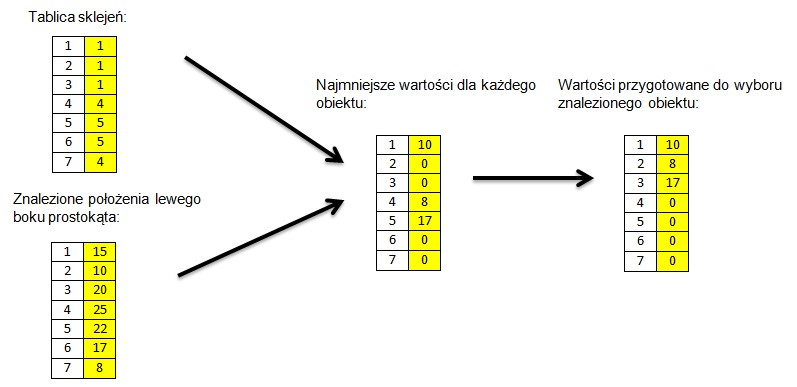
\includegraphics[width=\textwidth]{ind_schemat.jpg}
	\caption{Schemat procesu przetwarzania informacji po~każdej ramce obrazu z przykładowymi danymi. Tablica sklejeń daje informację o~konieczności sklejenia etyket 1, 2, 3. Ponieważ przykład dotyczy lewego boku prostokąta, spośród liczb 15, 10, 20 (odpowiadającym etykietom 1, 2, 3) wybierana jest najmniejsza. Ostatni krok przetwarzania to~usunięcie środkowych zer z~wektora.}
	\label{fig:ind_schemat}
\end{figure}
%TODO Schemat niejasny.(dodany opis)

Główną trudnością w~implementacji opisanego algorytmu w~układzie FPGA jest stosunkowo duże zapotrzebowanie na~zasoby sprzętowe. 
Należy zarezerwować miejsce na~cechy każdego potencjalnego obiektu. 
Ogranicza to~liczbę możliwych etykiet. 
Zarezerwowanie miejsca dla 30~obiektów nie~przekroczyło możliwości układu ZYBO. 
Badania pokazały, że~jest to wystarczająca liczba etykiet do~sprawnego działania toru wizyjnego i~ostatecznie zaimplementowano moduł w~tej wersji.\par
%TODO 1. Zostało to zaimplementowane ?
%TODO 2. Skoro indeksacja to po co wcześniejszy środek ciężkości (usunięty środek ciężkości)
\subsection{Wyznaczane informacje o detekcji}
\label{sec:informacje_o_detekcji}
Wyznaczanymi informacjami o~detekcji, koniecznymi do~realizacji algorytmu sterowania, są:
\begin{itemize}
	\item wartość bezwzględna uchybów regulacji w~obu osiach, rozumiana jako odległość środka obrazu od~centrum prostokąta otaczającego,
	\item ćwiartka układu współrzędnych, w~której znajduje się znacznik,
	\item wiadomość o~znalezieniu znacznika.
\end{itemize}
Dodatkowo, w~celu śledzenia działania systemu, istnieje możliwość podglądu przetworzonego obrazu na~monitorze, podłączonym poprzez HDMI. Możliwy jest podgląd kolejnych etapów przetwarzania; wybór etapu następuje przez zmianę ustawień przełączników na~płytce.\\
\subsection{Integracja płytki z autopilotem}
\label{sec:integracja_plytka_autopilot}
W~układzie ZYBO~Z7-20 wykorzystano interfejs UART0. Wyprowadzono piny TX i~RX z~systemu procesorowego i~podłączono je do~portu Pmod~JB. Po~stronie sterownika Pixhawk użyto portu TELEM~2. Szybkość transmisji to~115200~bodów.\\
Wysyłanie komend opiera się na~wykorzystaniu gotowych funkcji dostępnych w~sieci \cite{github_mavlink}. Przygotowują one daną wiadomość zgodnie z~wymaganiami protokołu MAVLink. Następnie wywoływane są funkcje wysyłające przygotowaną tablicę bajtów przez odpowiedni UART. W~projekcie wykorzystano stworzone przy wykonywaniu pracy \cite{mgr} funkcje opakowujące kolejne etapy przetwarzania komend.
%TODO Znacznik. Potem przestrzenie barw i reszta(wykonane w testach)
%-------------------------------------------------------------------------